\section{Data analysis and Validation}

\graphicspath{{Chapter3/Figs/}}

\begin{frame}
  \frametitle{Input Datasets}
  \framesubtitle{}
  \label{ch3:data}
  
  \textbf{For validation:}
  \begin{enumerate}
    \item EPN network, solution C2010 - ETRF 2014 (299 stations)
    \item EPOS network, INGV solution (571 stations)
    \item EPOS network, CNRS solution (MIDAS) (452 stations)
    \item network GREECE, NTUA reprocessing 2017 (153 stations)
  \end{enumerate}
    
\end{frame}
\note{}

\begin{frame}
  \frametitle{Validation}
  \framesubtitle{emax - emin maps comparison}
  \label{ch3:data}
  
  \begin{columns}
    \begin{column}{0.5\textwidth}
      VISR
      
      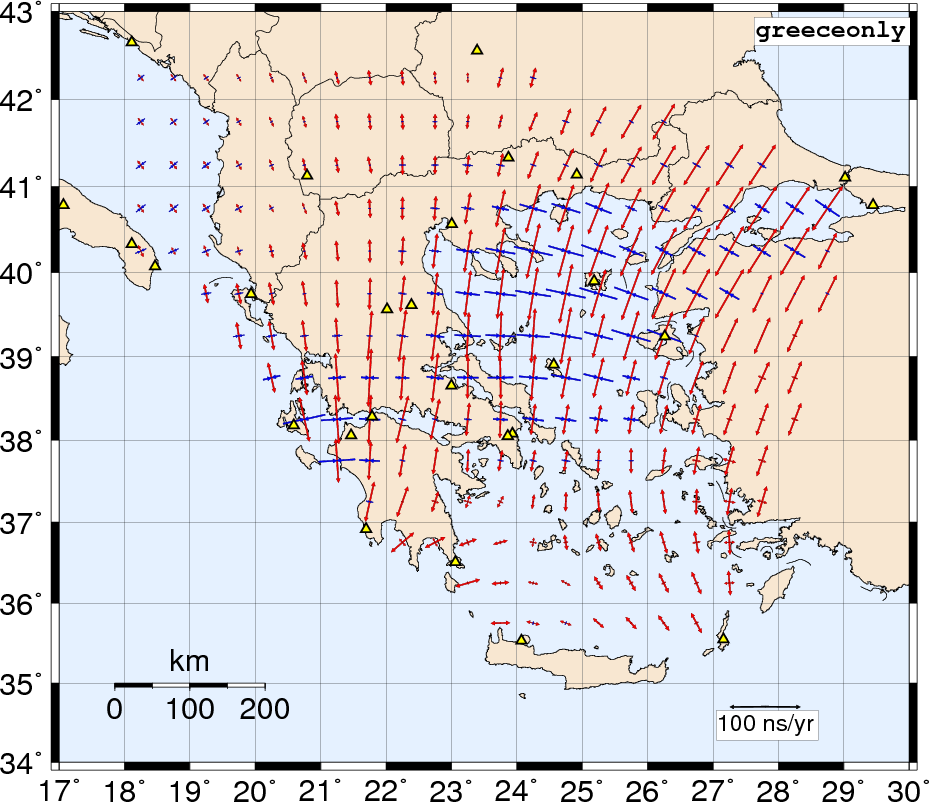
\includegraphics[width=.9\textwidth]{a1_map_strain_vectors.png}   
    \end{column}
    \begin{column}{0.5\textwidth}
    \begin{center}
      PyStrain
      
      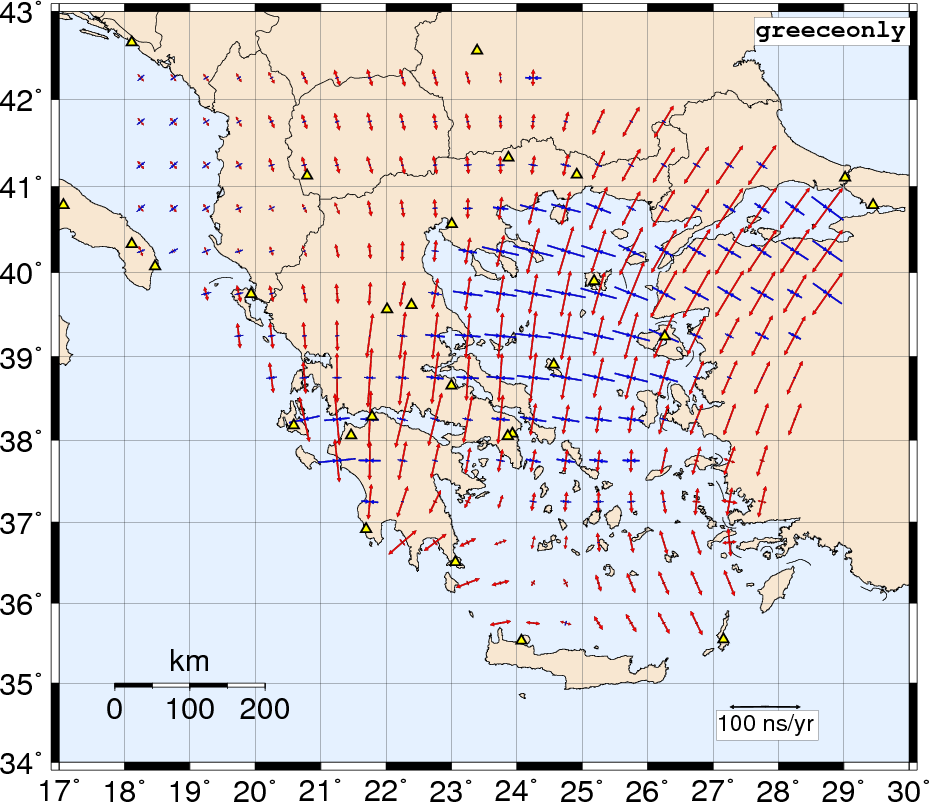
\includegraphics[width=0.9\textwidth]{a2_map_strain_vectors.png}     
    \end{center}
    \end{column}
  \end{columns}

\end{frame}
\note{}

\begin{frame}
  \frametitle{Validation}
  \framesubtitle{dilatation maps comparison}
  \label{ch3:data}
  
  \begin{columns}
    \begin{column}{0.5\textwidth}
      VISR
      
      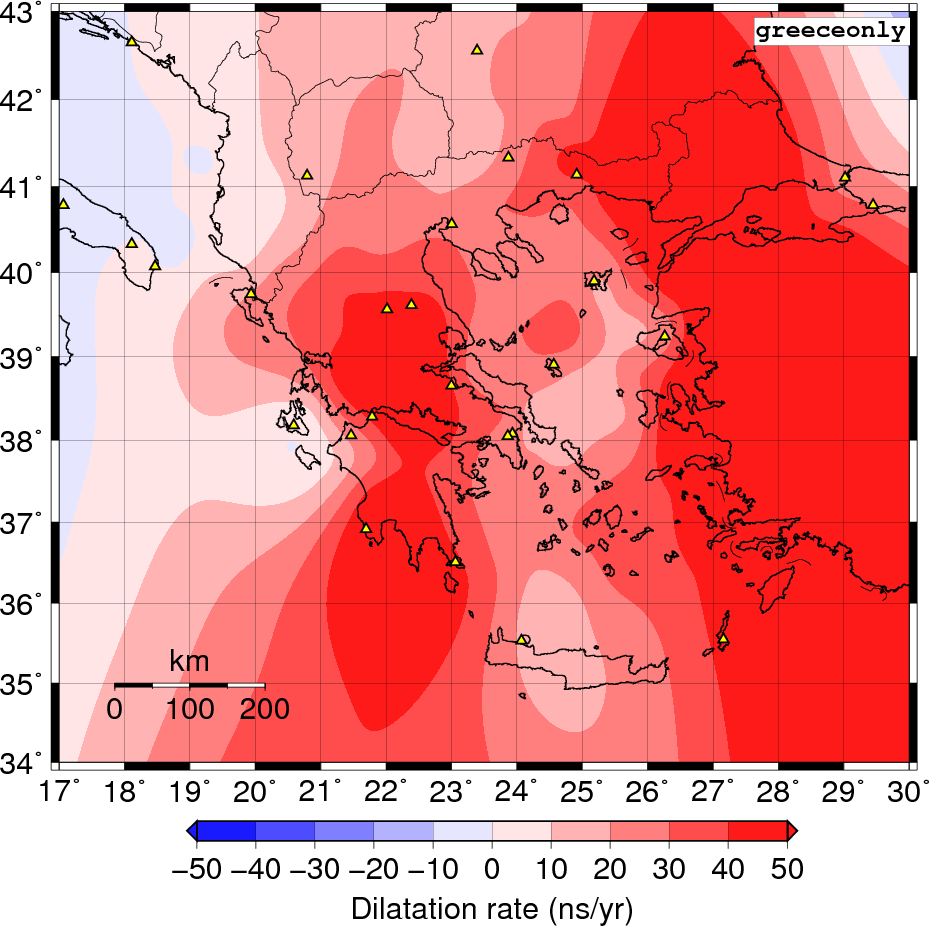
\includegraphics[width=.9\textwidth]{b1_map_strain_dilatation.png}   
    \end{column}
    \begin{column}{0.5\textwidth}
    \begin{center}
      PyStrain
      
      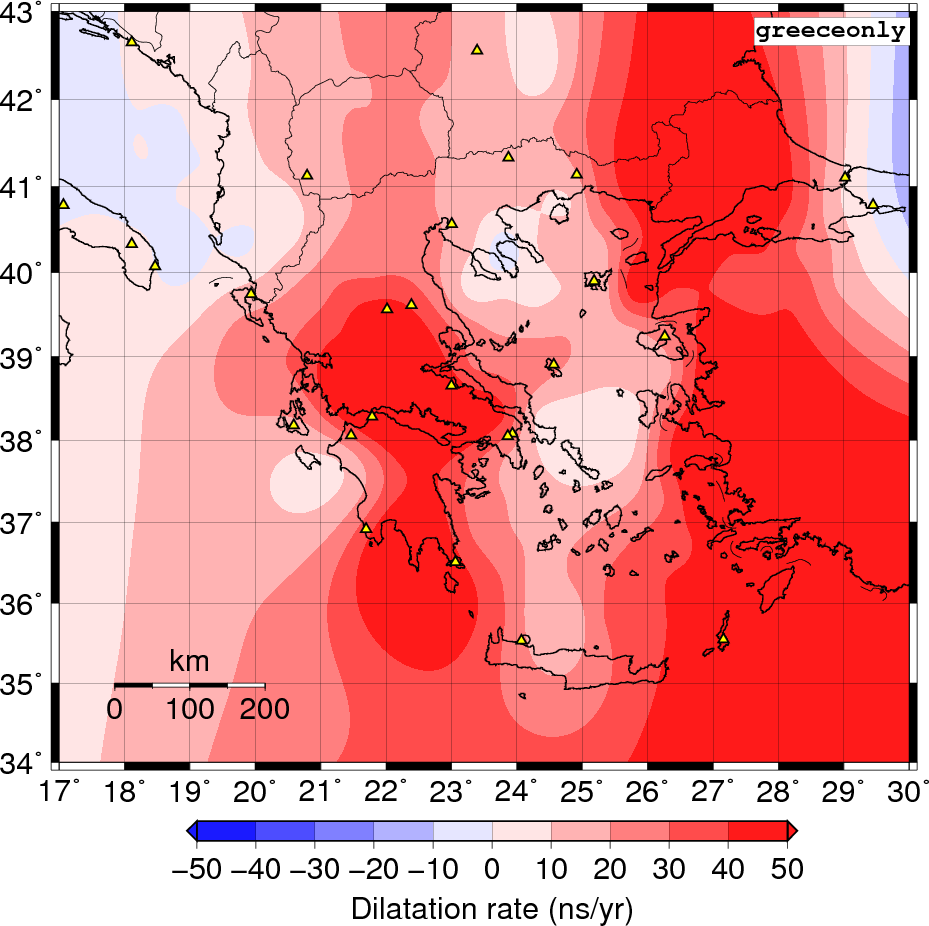
\includegraphics[width=0.9\textwidth]{b2_map_strain_dilatation.png}     
    \end{center}
    \end{column}
  \end{columns}

\end{frame}
\note{}



%\begin{frame}
%  \frametitle{Συμπεράσματα}
%  \framesubtitle{}
%  \label{ch3:}

%\end{frame}
%\note{}
